\section{Lezione 03 - 13/03/2023}

\subsection{Disposizioni}
\textbf{Disposizione:} è una selezione dove l'ordinamento è  \textbf{IMPORTANTE}.\\
Per calcolare tutte le k-disposizioni con ripetizione di S usiamo questa formula:
$$ D^{(r)}_{n,k} = n^k$$ 
%$$ D^{(r)}_{n,k} = n^k \: \: \: \: \: (k>=n)$$ 

Per calcolare tutte le k-disposizioni semplici di S usiamo questa formula:

$$ D_{n,k} = \frac{n!}{(n-k)!} \: \: \: \: \: (k<=n)$$ 

\begin{center}
($n$ cardinalità dell'insieme, $k$ la lunghezza della disposizione)
\end{center}
%Ora forniamo degli esempi per definire alcuni modi di formulare il calcolo combinatorio

\subsubsection{Esempio del gioco del Tris (Disposizione Semplice)}
Dati:
\begin{itemize}
\item 9 Cavalli in gara $\Rightarrow$ Alfabeto costituito da 9 valori
$S = \{C_1,..., C_n\}$
\item Si punta sul podio del cavallo quindi quante terne di cavalli posso avere \textbf{senza ripetizione} e \textbf{con ordine}.
\end{itemize}
Se un cavallo esce dalla terna allora non potrà ripresentarsi nella prossima posizione, quindi \textbf{senza ripetizione}.\\
Dunque quante sono le sequenze lunghe $k$ ($\le n$) composte dai simboli dell'alfabeto $S$.\\
Generalizzando abbiamo:	
$$ D_{n,k} = n(n-1)...(n-k) = \frac{n!}{(n-k)!} \: \: \: \: \: (k<=n)$$ 
%Dove $n,k \in N$ e $k\le n$

Questo tipo di calcolo combinatorio è chiamato \textbf{Disposizione /(semplice)}.\\


%Possiamo suddividerla in:\\
%Disposizione: è ammessa la \textbf{ripetizione} di qualunque %elemento\\
%Diposizione Semplice: \textbf{non è amessa} la ripezioni\\\\
%\textbf{Combinazioni: } è una selezione dove l'ordinamente %\textbf{non è IMPORTANTE}.\\
%Possiamo suddividerla in:\\
%Combinazioni: è ammessa la \textbf{ripetizione} di qualunque %elemento\\
%Combinazioni Semplice: \textbf{non è amessa} la ripezioni\\\\

\subsubsection{Esempio Totocalcio (Disposizione con Ripetezione)}
Consideriamo le schedine Totocalcio, in cui abbiamo $n$ righe in cui si può scomettere su due squadre, l'alfabeto è composta da:
$$ S =\{1,x,2\} $$
Quante sono tutte le schedine del totocalcio che si possono costruire sapendo che ci sono $11$ partite?\\
Ogni scomessa può avere $3$ valori possibili, quindi abbiamo $11$ caselle con ognuna $3$ possibili varianti.\\
Dato che \textbf{l'ordine conta} parliamo di \textbf{disposizioni} e le ripetizione sono ammesse, quindi possiamo usare la "vecchia" regola moltiplicativa cioé: $n^k$, quindi le disposizione con ripetizione:\\
$$ D^{(r)}_{n,k} = n^k = 3^11 = 177147$$ 

\subsubsection{Esempio di Disposizione}
Poniamo caso di voler sapere le possibili di dispozioni normali e semplici di un dato insieme di lettere.
Per semplicità consideriamo l'insieme $S=\{c,a\}$, poniamo caso che vogliamo sapere tutte le possibili parole di lunghezza $2$.\\
Quindi $n = \#S = 2$ e $k = 2$, allora:

$$ D^{(r)}_{n,k} = n^k = 2^2 = 4 = \{(c,c),(a,a),(c,a),(a,c)\} $$
$$ D_{n,k} = \frac{n!}{(n-k)!} = \frac{2!}{0!} = 2! = 2 = \{(c,a), (a,c)\}$$ 

\subsection{Permutazioni}
Ogni n-disposizione semplice è detta una permutazione degli n elementi di S\\
(Possiamo considerare le permutazioni un caso speciale delle 
\hyperref[sec:disposizioni]{disposizioni semplici}, cioè avviene quando $n=k$)
$$ (se \: k=n) \: \: \: P_n = D_{n,n} = \frac{n!}{\equalto{(n-n)!}{0!=1}} = n!  $$

\subsection{Permutazioni con Ripezioni}
Sia $n=k_1+k_2+...+k_r$, Una n-selezione di S avente $k_1$ elementi uguali al primo elemento di S, $k_2$ elementi uguali al secondo elemento di S e cosi via fino a $k_r$ è detta una $(k_1,k_2,...,k_r)$-permutazioni con ripetizioni.\\
Il numbero di tutte le $(k_1,k_2,...,k_r)$-permutazioni con ripetizioni di S è dato da:
$$ P^{(r)}_n = \frac{n!}{k_1! * k_2! * ... * k_r!} = \binom{n}{k_1,...,k_r} \: \: (k_1+...+k_r)=r$$

\subsection{Esempi Permutazioni}
$$ S=\{A,I,O,S\} \: \#S=4 \: k=n=4  $$
Possiamo formare varie parole: OASI, SAIO, SOIA..., possiamo calcolarle:
$$ P_4 = 4! = 24  $$

Poniamo caso che vogliamo sapere le possibili combinazioni di $STATISTICA$, possiamo notare che più lettere si ripetono quindi mettiamo al denomitore il numero di volte che la lettere che si ripete al fattoriale, per calcore dobbiamo usare:
$$ _{n_1,n_3,n_3,...,n_r}P_n \frac{10!}{2!3!2!2!1!} $$
il $10!$ si riferisce alla lunghezza della parola.

\subsection{Combinazioni Semplici}
Sia $k<=n$, una k-combinazione semplice di S si ottine indentificando tutte le k-disposizioni semplici di S senza dare importanza all'ordine.\\
Il numero di tutte le k-combinazioni semplici è dato da:
$$ C_{n,k} = \binom{n}{k} \: \: \: (con\:k<=n)$$

\subsubsection{Esempio Ruota di Napoli (Combinazione Semplici)}
Il gioco consiste nell'estrarre tre numeri da un alfebeto: $S=\{1,2,...,90\}$, i numeri estratti non possono ripetersi e l'ordine non è importante.\\
In questo caso dato che l'ordine non conta le disposizioni ci danno un numero troppo grande quindi dobbiamo andare a rimuovere le parte in eccesso:
$$ \frac{D_{90,3}}{P_3} = \frac{90!}{(90-3)!}*\frac{1}{3!} = \frac{90!}{87! 3!} = \binom{90}{3} = C_{90,3} $$
Quindi quando parliamo di sequenza senza ordine useremo il termine \textbf{combinazioni} in questo caso semplici poiché non cononta l'ordine.

\subsection{Combinazioni con Ripetizioni}
Una k-combinazione con ripetizione di S si ottiene identificando tutte le k-disposizioni con ripetizioni di S aventi i medesii elementi posti in un differente ordine (in altri termini è ammessa la ripetizioni di qualche elemento di S e l'ordine è ininfluente).\\
Il numero di tutte le k-combinazioni con ripetizioni di S è dato da:
$$ C_{n,k}^{(r)} = \binom{n+k-1}{k} $$

\newpage

\subsection{Recap}
Piccolo recap di tutte le formule:
\begin{itemize}
\item Disposizioni con Ripetizioni: $D^{(r)}_{n,k} = n^k$
\item Disposizioni senza Ripetizioni: $ D_{n,k} = \frac{n!}{(n-k)!} \: \: \: \: \: (k<=n) $
\item Permutazioni con Ripetizioni: $P^{(r)}_n = \binom{n}{k_1,...,k_r} \: \: (k_1+...+k_r)=r$
\item Permutazioni senza Ripetizioni: $P_n = n!$
\item Combinazioni con Ripetizioni: $ C_{n,k}^{(r)} = \binom{n+k-1}{k} $
\item Combinazioni senza Ripetizioni: $ C_{n,k} = \binom{n}{k} \: \: \: (con\:k<=n) $
\end{itemize}
\begin{center}
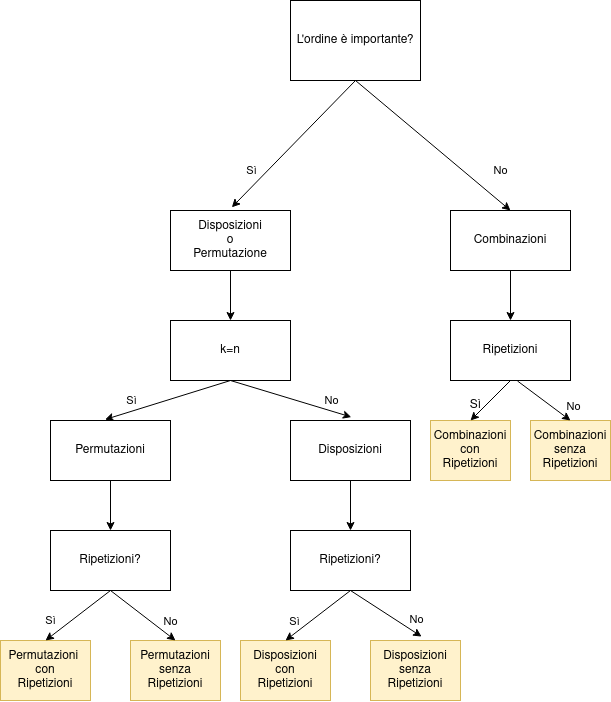
\includegraphics[width=0.8\textwidth]{schema}
\end{center}
%\includesvg{Lezioni/DisposizioniPermutazioniCombinazioni.drawio.svg}


